\chapter{Literature Review}

This chapter contains a review of traditional approaches to AI in video games.
It then explores RL and deep learning fundamentals, algorithms and data structures, as well as some of their existing applications to video games.

\section{Traditional approaches to AI in video games}

This section explores some existing traditional methods of implementing AI in video games.

\subsection{Finite State Machines}

A Finite State Machine (FSM) is a computational model that has been foundational in video game AI development for decades. 
FSMs represent an agent's behavior as a set of discrete states, with well-defined transitions between these states triggered by specific conditions or events \cite{spiceworks_fsm}. 

\begin{figure}[H]
    \centering
    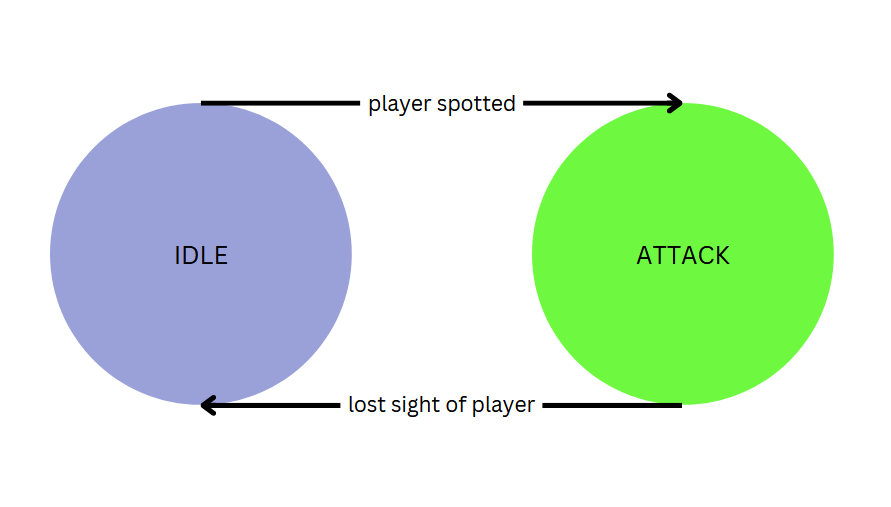
\includegraphics[width=0.8\textwidth]{figures/fsm_example.png}
    \caption{A simple FSM for an enemy NPC}
    \label{fig:fsm}
\end{figure}

Each state encapsulates a particular behavior or action pattern, while transitions define the rules governing when an agent should change its behavior. 
The simplicity and predictability of FSMs make them particularly suitable for controlling NPCs with straightforward behavioral patterns, as they are computationally efficient and easily debuggable.
However, FSMs face significant limitations as complexity increases: the number of states and transitions can grow exponentially, leading to the "state explosion" problem that makes maintenance challenging.
Additionally, FSMs struggle with handling concurrent behaviors and can appear rigid when compared to more dynamic AI approaches. 
Despite these limitations, FSMs remain prevalent in game development due to their intuitive implementation and reliable performance for many common AI tasks.

\subsection{Behaviour Trees}

Behaviour Trees (BTs) represent a significant advancement over FSMs in game AI architecture, offering a hierarchical, modular approach to decision-making. 
Originally developed for robotics and adopted by the game industry in titles like Halo 2 \cite{simulacrum}, BTs organize agent behaviors into a tree structure where leaf nodes represent atomic actions and internal nodes control flow through various composites such as sequences, selectors, and parallels. 
This structure enables developers to create complex, reusable behavior patterns that can be visually represented and intuitively understood. 
Unlike FSMs, BTs naturally handle concurrent actions and gracefully manage behavior prioritization through their hierarchical evaluation.
BTs excel at creating responsive AI that can react to changing game conditions while maintaining coherent behavior patterns. 
They facilitate an incremental development approach, allowing designers to progressively refine AI by adding branches without disrupting existing functionality.
While BTs require more initial design consideration than FSMs, their scalability, maintainability, and ability to represent sophisticated decision-making logic have made them the standard approach for contemporary game AI systems, particularly in action, strategy, and open-world games where adaptable NPC behavior is critical to player experience.

\begin{figure}[H]
    \centering
    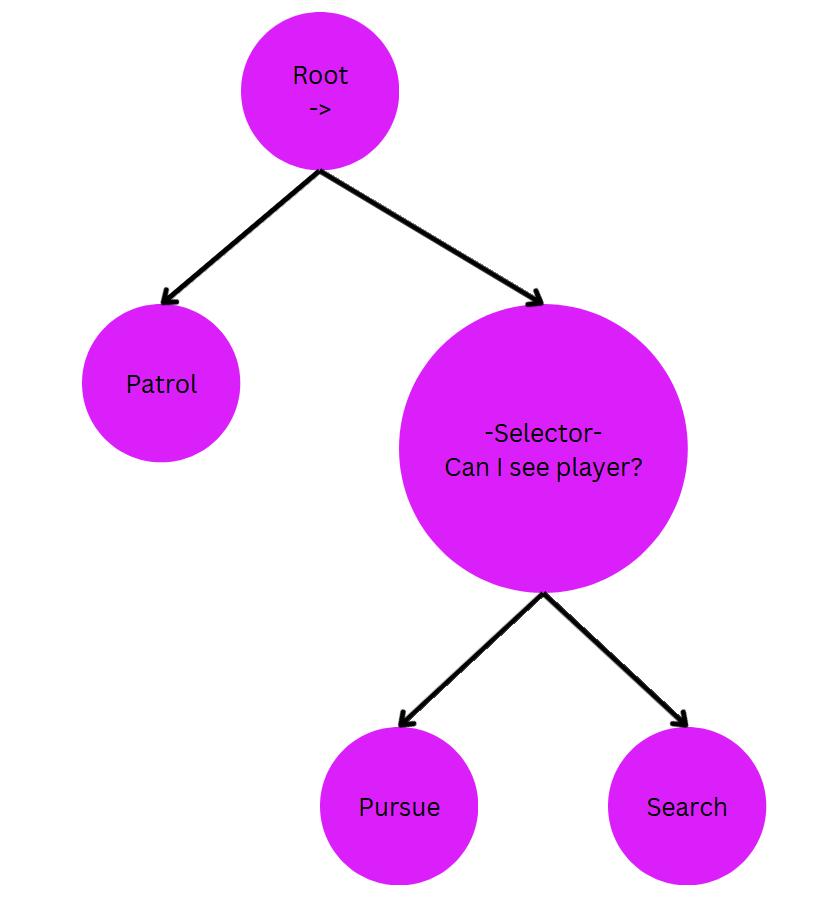
\includegraphics[width=0.8\textwidth]{figures/bt.png}
    \caption{A simple BT for an enemy NPC}
    \label{fig:bt}
\end{figure}

\subsection{Goal-Oriented Action Planning}

Goal-Oriented Action Planning (GOAP) represents a more dynamic approach to AI decision-making compared to FSMs and BTs. 
GOAP employs principles from automated planning and means-end analysis to create AI agents that formulate plans to achieve specific goals. Unlike more rigid systems, GOAP agents dynamically determine action sequences by considering current world states, available actions with preconditions and effects, and desired goal states.
In a GOAP system, each action is associated with both preconditions (requirements that must be satisfied before the action can be taken) and effects (how the action changes the world state).
The AI agent uses planning algorithms, commonly A* search, to find the optimal sequence of actions that transforms the current state into the goal state. 
This approach allows NPCs to solve problems creatively and adapt to unexpected changes in the game environment.
GOAP gained prominence through its implementation in F.E.A.R. (2005) \cite{thompson2020fear}, where it produced enemies capable of contextually appropriate tactical behaviors like seeking cover, flanking the player, and coordinating with allies. 
The system's strength lies in its separation of goals (what the agent wants to achieve) from the specific methods to achieve them, creating emergent behavior that can surprise even the developers.
While GOAP offers exceptional adaptability and problem-solving capabilities, it comes with higher computational costs and increased implementation complexity compared to FSMs and BTs. Despite these challenges, GOAP remains valuable for games requiring sophisticated AI that can respond intelligently to dynamic and unpredictable gameplay scenarios.

\begin{figure}[H]
    \centering
    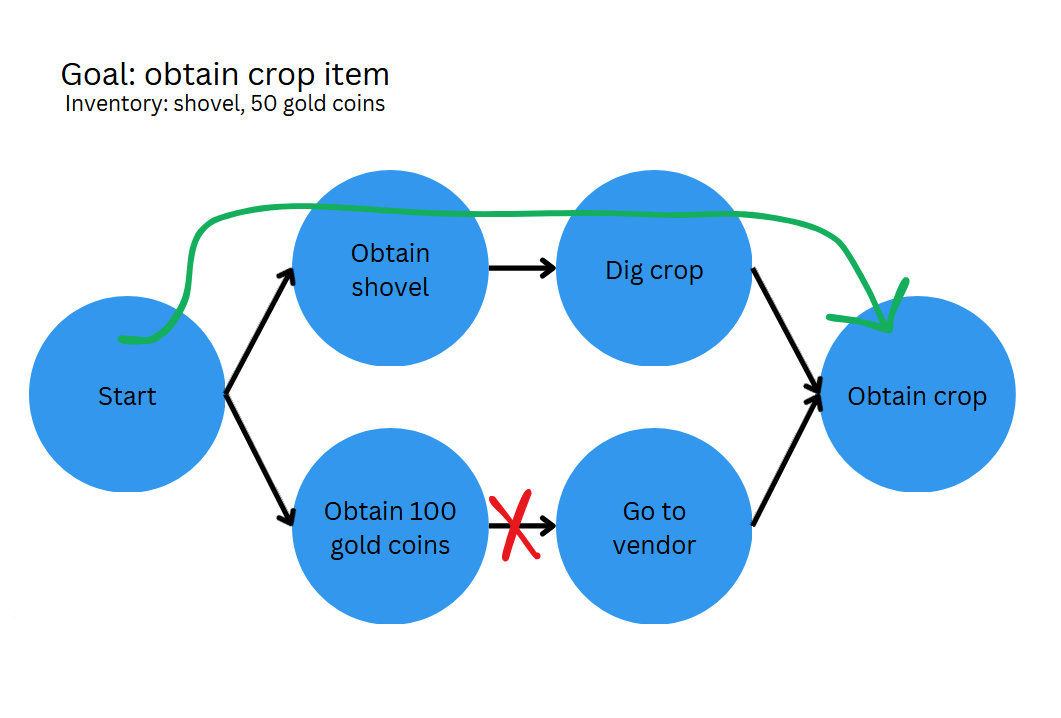
\includegraphics[width=0.8\textwidth]{figures/goap.png}
    \caption{Example of a GOAP planning sequence}
    \label{fig:goap}
\end{figure}

\section{Reinforcement Learning}

This section explores fundamental RL concepts and algorithms.

\subsection{RL Fundamentals and the Markov Decision Process}

Reinforcement Learning (RL) represents a departure from traditional game AI approaches by focusing on learning optimal behaviors through trial and error interaction with an environment. 
Unlike FSMs, BTs, or GOAP systems that rely on pre-programmed rules, RL agents improve their decision-making capabilities through experience.

At its core, RL is formalized as a Markov Decision Process (MDP) consisting of:
\begin{itemize}
    \item A set of states $S$ representing all possible situations an agent may encounter
    \item A set of actions $A$ that the agent can take
    \item Transition probabilities $P(s'|s,a)$ defining the likelihood of moving to state $s'$ after taking action $a$ in state $s$
    \item A reward function $R(s,a,s')$ providing feedback on the quality of decisions
    \item A discount factor $\gamma \in [0,1]$ determining the importance of future rewards
\end{itemize}

\begin{figure}[H]
    \centering
    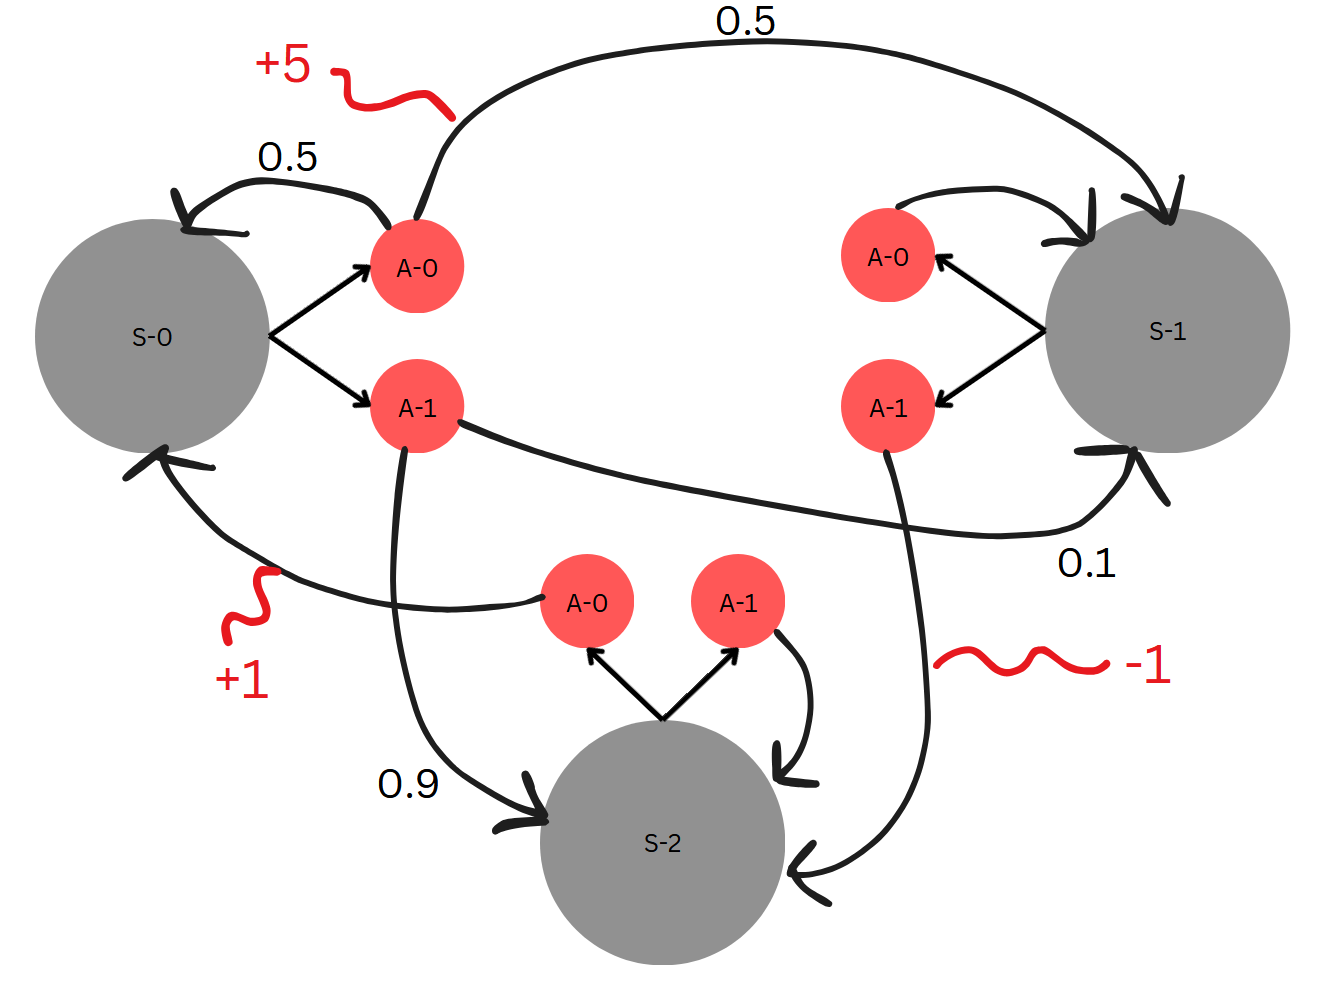
\includegraphics[width=0.8\textwidth]{figures/mdp_framework.png}
    \caption{A simple MDP Graph example}
    \label{fig:mdp-framework}
\end{figure}

S Nodes represent states and A nodes represent actions. 
Some actions can result in more than one state, the transition probabilities are marked in black. 
Some actions result in a positive or negative reward, marked in red.

The agent's objective is to learn a policy $\pi$ that maps states to actions in a way that maximizes the expected cumulative reward. 
This optimisation process balances immediate rewards against long-term consequences, addressing the fundamental exploration-exploitation dilemma: whether to capitalize on known good strategies or explore new possibilities that might yield better results.
RL algorithms generally fall into three categories: value-based methods (like Q-learning), policy-based methods (such as policy gradients), and actor-critic approaches that combine aspects of both. 
The choice of algorithm depends on factors including the complexity of the state space, whether the environment is fully observable, and computational constraints.
Unlike traditional AI techniques, RL offers adaptability to unexpected situations and can discover novel strategies beyond designer expectations. 
However, these advantages come with challenges including high sample complexity (requiring many environment interactions), difficulty in specifying appropriate reward functions, and potential convergence to suboptimal solutions when trained in limited scenarios.

\subsection{Deep Reinforcement Learning}

Deep Reinforcement Learning (DRL) combines classical RL with deep neural networks to handle high-dimensional state spaces that would be intractable with traditional tabular methods. 
This integration enables RL to operate effectively in complex environments with visual inputs, continuous action spaces, and intricate state representations common in modern video games.

The breakthrough Deep Q-Network (DQN) algorithm, introduced by DeepMind in 2015, demonstrated superhuman performance on Atari games using only pixel inputs and game scores. DQN employs several key innovations including:
\begin{itemize}
    \item Experience replay, which stores and randomly samples past experiences to break correlation between sequential samples
    \item Target networks that stabilize training by reducing moving target problems
    \item Convolutional neural networks that process visual information effectively
\end{itemize}

\begin{figure}[H]
    \centering
    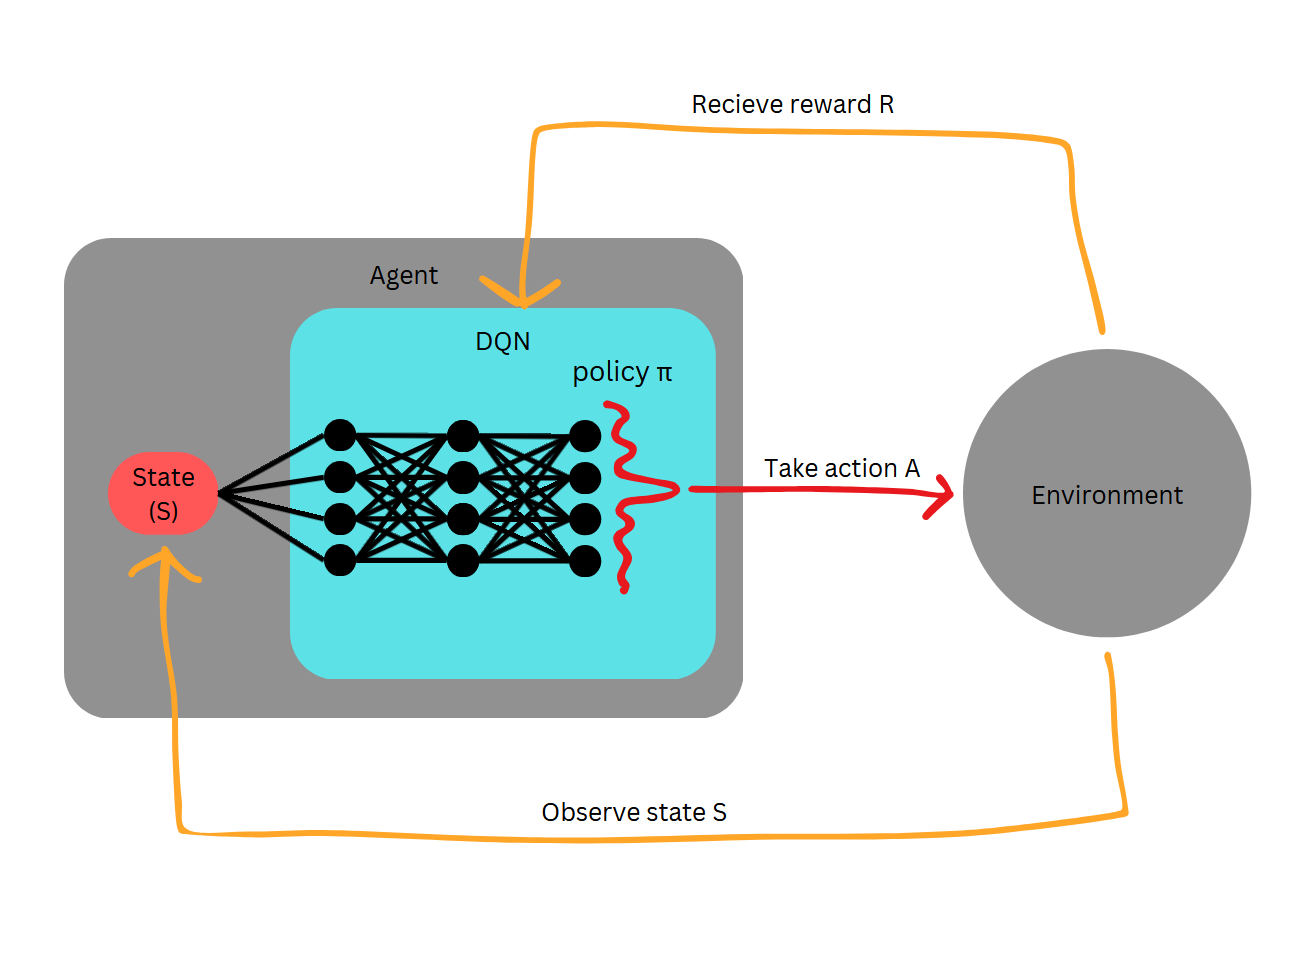
\includegraphics[width=0.8\textwidth]{figures/dqn_architecture}
    \caption{Architecture of a Deep Q-Network}
    \label{fig:dqn-architecture}
\end{figure}